Sourdough has been made since ancient times. The exact origins of fermented
bread are, however, unknown. One of the most ancient preserved
sourdough breads has been excavated in Switzerland.
However, based on recent research, some scientists speculate that sourdough
bread had already been made in 12000 BC in ancient Jordan \cite{jordan+bread}.

\begin{figure}[h]
  \includegraphics[width=\textwidth]{cover-page}
  \caption{.jpg works}
\end{figure}

\begin{figure}[h]
  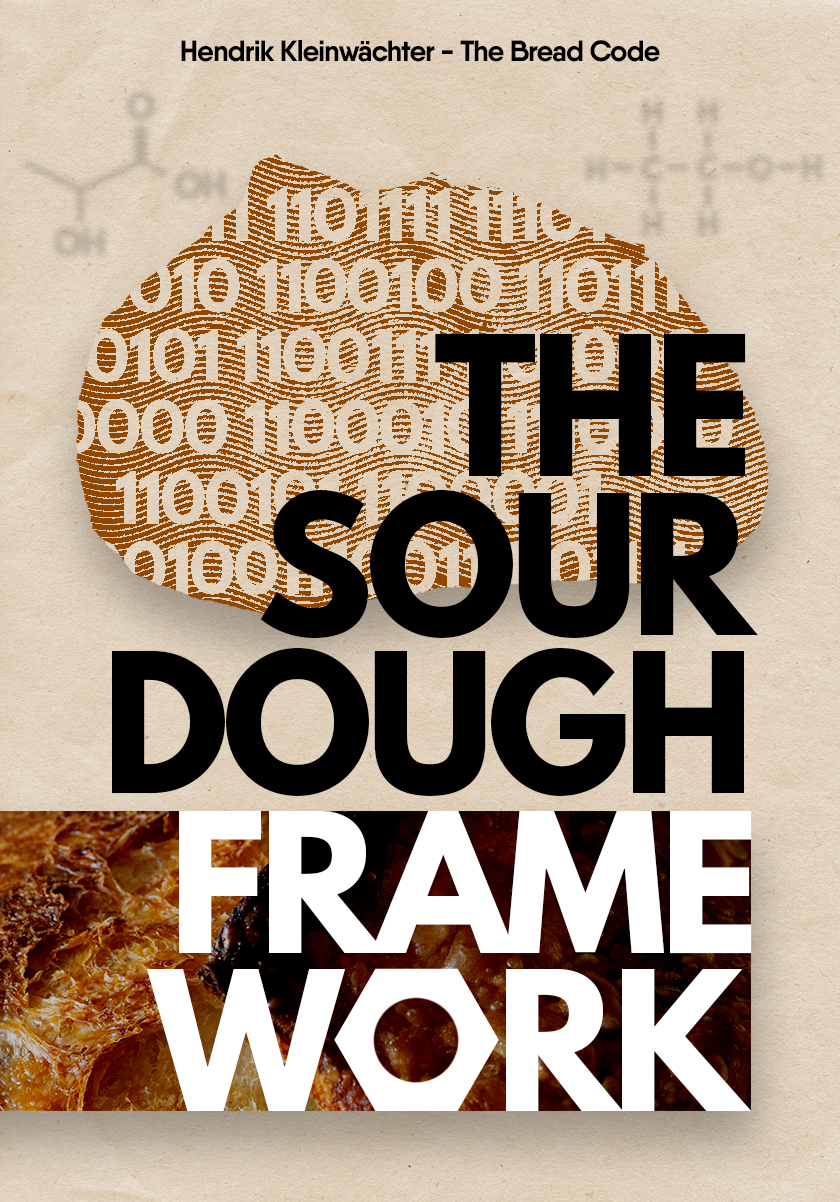
\includegraphics[width=\textwidth]{cover-page-2}
  \caption{.jpg duplicated not working}
\end{figure}

\begin{figure}[h]
  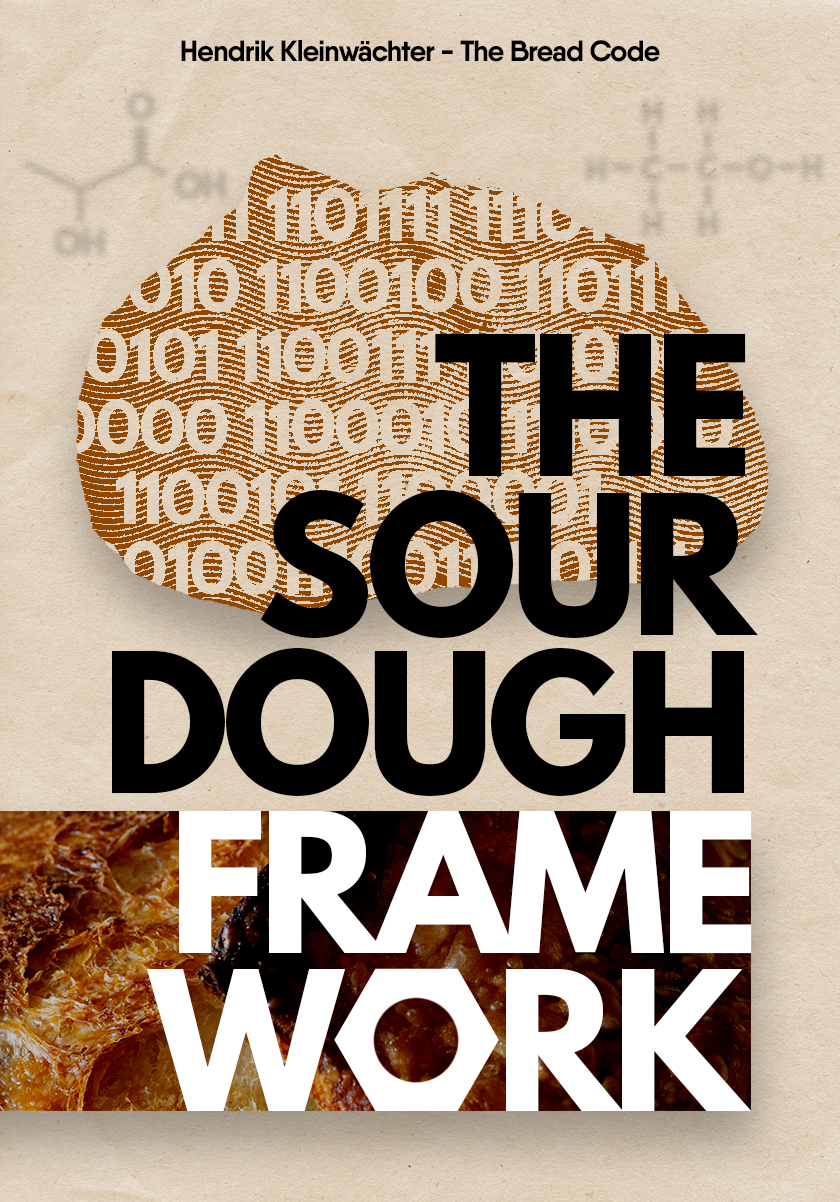
\includegraphics[width=\textwidth]{foobar}
  \caption{simple filename test .foobar}
\end{figure}

\begin{figure}[h]
  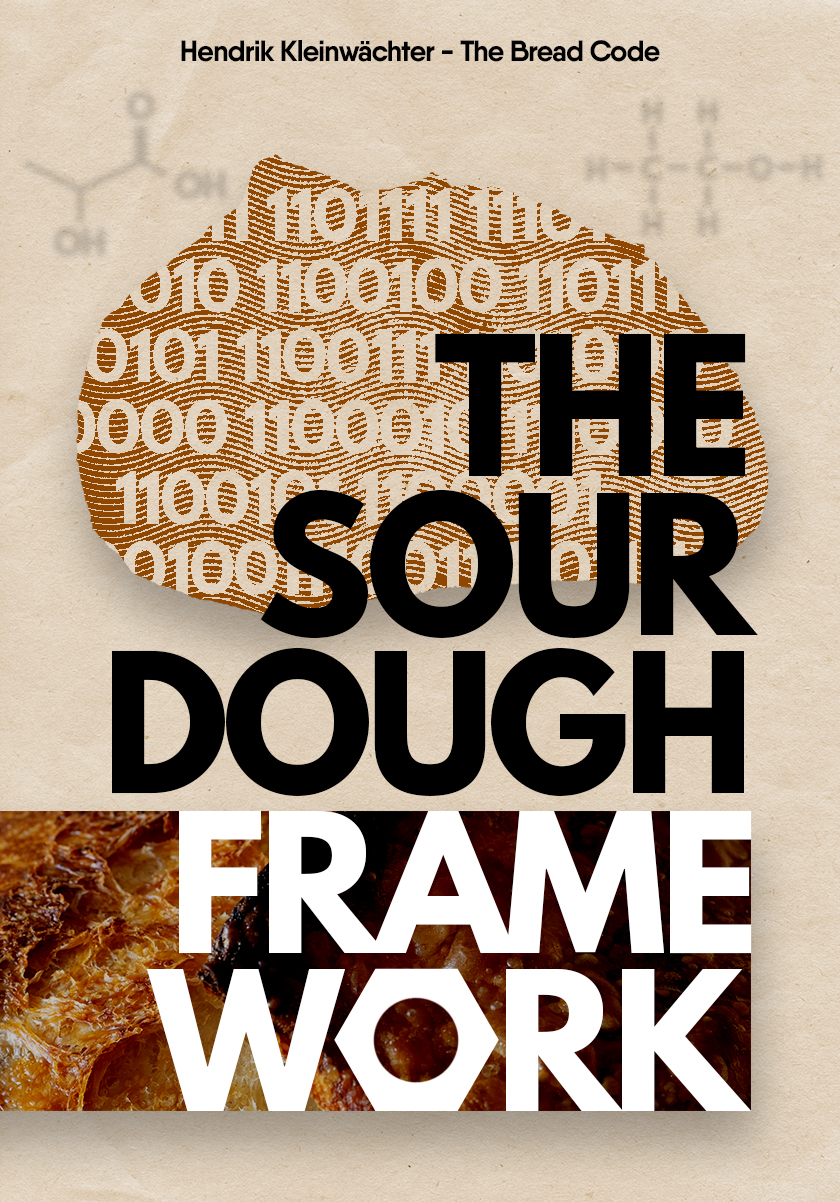
\includegraphics[width=\textwidth]{cover-page-3}
  \caption{.png not working}
\end{figure}

Another popular story is that a lady in Egypt was making
a bread dough close to the Nile river. The lady forgot the
dough and returned a few days later. She noticed that the dough had
increased in size and smelled funky. She decided to bake
the dough anyway. She was rewarded with a much
lighter, softer, better tasting bread dough. From that day
on she continued to make bread this way.

Little did the people back then know that tiny microorganisms
were the reason they made better bread. It is not clear when
people started using a bit of the dough from the previous
day for the next batch of dough. But by doing so, sourdough
bread making was born. Wild yeast in the flour and in the air
plus bacteria start to decompose the flour-water mixture, also
known as your dough. The yeast makes the dough fluffy and
the bacteria primarily creates acidity. The different
microorganisms work in a symbiotic relationship. Humans
appreciated the enhanced airy structure and slight acidity
of the dough. Furthermore, the shelf life of such bread
was extended due to the increased acidity. 

Quickly, similar processes were discovered when brewing beer
or making wine. A small tiny batch of the previous production
would be used for the next production. In this way, humans created
modern bread yeasts, wine yeasts, and beer yeasts. Only in 1680,
the scientist scientist Anton van Leeuwenhoek first studied yeast microorganisms
under a microscope. Over time with each batch, the yeasts and bacteria
would become better at consuming whatever they were thrown at.
By feeding your sourdough starter you are selectively breeding
microorganisms that are good at eating your flour. With
each iteration, your sourdough knows how to better ferment the flour
at hand. This is also the reason why more mature sourdough starters sometimes
tend to leaven doughs faster (source needed). It is crazy if you
think about it. People have been using this process despite not
knowing what was actually going on for thousands of years! The
sourdough in itself is a symbiotic relationship. But the sourdough
also adapted to humans and formed a symbiotic relationship with us.
For food and water, we are rewarded with delicious bread. In exchange,
we shelter and protect the sourdough. Spores from the starter
are spread through aerial contamination or insects like fruit flies.
This allows the sourdough starter to spread its spores even
further all around the world. 

Brewers would start to experiment with utilizing the muddy leftovers
of the beer fermentation to start making doughs. They would notice
that the resulting bread doughs were becoming fluffy and compared
to the sourdough process would lack the acidity in the final product.
A popular example is shown in a report from 1875. Eben Norton Horsford
wrote about the famous "Kaiser Semmeln" (Emperor's bread rolls).
These are essentially bread rolls made with brewer's yeast instead
of the sourdough leavening agent. As the process is more expensive,
bread rolls like these were ultimately consumed by the noble people
in Vienna \cite{vienna+breadrolls}.

\begin{figure}[h]
  \includegraphics[width=\textwidth]{sourdough-stove}
  \caption{A bread made over the stove without an oven}
  \label{sourdough-stove}
\end{figure}

Only in 1857, the French microbiologist Louis Pasteur discovered
the process of alcoholic fermentation. He would prove that
yeast microorganisms are the reason for alcoholic fermentation
and not other chemical catalysts. What would then start is
what I describe as the 150 lost years of bread making. In 1879
the first machines and centrifuges were developed to centrifuge
pure yeast. This yeast would be extracted from batches of sourdough.
The pure yeast would prove to be excellent and turbocharged
at leavening bread doughs. What would previously take 10 hours
to leaven a bread dough could now be done within 1 hour.
The process became much more efficient. During world war II
the first packaged dry yeast was developed. This would ultimately
allow bakeries and home bakers to make bread much faster.
Thanks to pure yeast, building bread making machines was
possible. Provided you maintain the same temperature
your yeast would always ferment exactly the same way. As fermentation
times sped up the taste of the final bread would deteriorate.
The sprouting process induced by certain enzymes is essential
to developing a fluffier texture and better tasting crust. This
can't be indefinitely sped up. Soon bakeries would start
to introduce additional enzymes to achieve similar properties
to sourdough bread in yeast-based doughs. Sourdough almost completely
vanished from the surface of the Earth. Only a handful
of true nerds would continue making bread with sourdough.
Suddenly people started to talk more often about celiac disease
and the role of gluten. The disease isn't new, it has first
been described in 250 AD \cite{coeliac+disease}. People
would note how modern bread has much more gluten compared
to ancient bread. The bread in ancient times probably was much flatter.
The grains over time have been bred more and more towards containing a higher
amount of gluten. Gluten is a protein that gives modern
bread its typical soft fluffy crumb structure. The
gluten proteins bind together once activated with water.
Throughout the course of the fermentation, CO2 is trapped
in this protein matrix. The tiny created chambers expand
during the baking process. As the dough gelatinizes while
being heated the structure is fortified. This makes the bread appear
soft and fluffy when tasting it. Similar to drinking raw cow's milk,
your immune system might react to the consumed proteins.
There is gluten intolerance
and celiac disease. When people say they don't handle
gluten well it's mostly a gluten intolerance they describe.
Some people describe similar issues when consuming
too much lactose. If you eat a long-fermented cheese
however most of the lactose has been fermented by
the tiny microorganisms. People would investigate and
note how sourdough bread can typically be handled better
compared to plain fast made factory bread. The
reason for this is that enzymes take time to work the dough.
Gluten is a storage protein of flour. Once
sprouting is activated by adding water, the protease
enzyme starts to convert the gluten into tinier amino acids
that are required for sprouting. Over time you are effectively
losing gluten as it's naturally broken down. Furthermore,
traditionally lactic acid bacteria would start to decompose
the flour-water mix. Almost everything is recycled in nature.
Part of their diet is to consume the proteins in the dough.
Modern bread is faster and no longer has lactic acid bacteria.
Both factors together mean that you are consuming products
with a much higher gluten value compared to ancient times
when natural fermentation was used \cite{raffaella+di+cagno}.

During the California Gold Rush, French bakers brought the sourdough
culture to Northern America. A popular bread became the
San Francisco sourdough. It's characterized by its unique
tang (which was previously common for every bread). It
however remained more of a niche food. What really expedited
the comeback of sourdough was the 2020 COVID-19 pandemic.
Flour and yeast became scarce in the supermarkets. While
flour returned yeast couldn't be found. People started
to look for alternatives and rediscovered the ancient
way of making sourdough bread. Soon many realized
that making sourdough bread is more complex than modern
yeast-based bread. You need to maintain a sourdough starter
and have it in ideal shape to properly ferment your dough.
Furthermore compared to a yeast-based dough you can't just
punch the dough down and let the fermentation continue.
You can overferment your dough, resulting in a sticky
dough mess. This complexity lead to many bakers looking
for help and many thriving communities formed around
the topic of homemade bread.

When interviewing Karl de Smedt (owner of the Sourdough
Library) he said something that changed my way of thinking
about bread: "The future of
modern bread is in the past \cite{interview+karl+de+smedt}."
